\section{Auswertung}
\label{sec:Auswertung}
\subsection{Fourier-Analyse: Fourier-Transformation}
Das Signal des Funktionsgenerator wird mit dem Oszilloskop angezeigt und es hat sich für jede Spannung ein Frequenzspektrum wie in Abbildung \ref{fig:linienspektrum} dargestellt, der hier in der Auswertung leider nicht zu sehen ist. 
\subsubsection{Rechteckspannung}
In der Tabelle \ref{tab:RechteckAnalyse} befinden sich die aufgeführten Werte für die Amplitude der Teilschwingungen. Die theoretischen Werte wurden nach der Formel \ref{eqn:Spannungungerade} bestimmt.
Die Abweichung errechnet sich nach:
\begin{equation}
\label{eqn:Abweichung}
a= \left|\frac{a_\text{theorie}-a_\text{gemessen}}{a_\text{theorie}}\right| \cdot \SI{100}{\percent}
\end{equation}
Das theoretische Verhältnis wird mit der folgenden Formel bestimmt:
\begin{equation}
\label{eqn:theoVerhalt}
U_{i} = \frac{100}{n}
\end{equation}
wobei $n$ der Kanal der jeweiligen Amplituden ist und $i = 1, 2, ...$ ist. 
Das prozentuale Verhältnis errechnet sich nach:
\begin{equation}
\label{eqn:prozVerhalt}
U_{i} = \frac{U_\text{gemessen}}{U_1}
\end{equation}
wobei $U_\text{gemessen}$ einfach die gemessenen Daten für jeden Kanal sind.
\begin{table}[htbp]
	\centering
	\caption{Rechteck: Gemessene Daten, theoretisches und prozentuales Verhältnis sowie die Abweichung $a$ in Prozent}
	\label{tab:RechteckAnalyse}
	\begin{tabular}{c c c c c c}
	\toprule
	$n$ & gemessene $U$/$\si{V}$ & theoretische $U$/$\si{V}$ & Prozent. Verhält. & Theo. Verhält. & Abweichung $a$ \\
	\midrule
		1 & 456 & 456 & 100 & 100 & 0 \\
		3 & 76 & 152 & 16,60 & 33,33 & 50,00 \\
		5 & 64 & 91,20 & 10,53 & 20,00 & 47,36 \\
		7 & 28 & 65,10 & 6,14 & 14,29 & 56,99 \\
 		9 & 20 & 50,60 & 4,39 & 11,11 & 60,47 \\
	\bottomrule
	\end{tabular}
\end{table}
\FloatBarrier
\subsubsection{Dreieckspannung}
In der Tabelle \ref{tab:DreieckAnalyse} befinden sich die gemessenen Daten für die Amplitude der Teilschwingungen.
Für die Berechnung der theoretichen Werte bei der Dreieckspannung wird aus Kapitel \ref{sec:Durchführung} die Formel \ref{eqn:SpannungDreieck} benötigt. Das prozentuale Verhältnis und das theoretische Verhältnis werden nach den Formeln \ref{eqn:theoVerhalt} und \ref{eqn:prozVerhalt} berechnet.
\begin{table}[htbp]
	\centering
	\caption{Dreieck: Gemessene Daten, theoretisches und prozentuales Verhältnis sowie die Abweichung $a$ in Prozent}
	\label{tab:DreieckAnalyse}
	\begin{tabular}{c c c c c c}
		\toprule
		$n$ & gemessen $U$/$\si{V}$ & theoretische $U$/$\si{V}$ & Prozent. Verhält. & Theo.Verhält. & Abweichung $a$ \\
		\midrule
		1 & 254 & 254 & 100 & 100 & 0 \\
		3 & 30 & 25,2 & 11,81 & 11,11  & 19,05 \\
		5 & 10 & 10,16 & 3,93 & 4,00 & 1,57 \\
		7 & 20 & 5,18 & 0,78 & 2,04 & 61,39 \\
		9 & 0 & 3,13 & 0 & 1,23 & 100 \\
		\bottomrule
	\end{tabular}
\end{table}
\FloatBarrier
\subsubsection{Sägezahnspannung}
In der Tabelle \ref{tab:SägezahnAnalyse} befinden sich ebenfalls die aufgeführten Werte für die Amplitude der Teilschwingungen. Analog werden hier die Berechnungen für das theoretische und prozentuale Verhältnis mit den Formeln \ref{eqn:prozVerhalt} und \ref{eqn:theoVerhalt} durchgeführt. Für die theoretischen Werte bei der Sägezahnspannung wird die Formel \ref{eqn:Spannungungerade} aus Kapitel \ref{sec:Durchführung} benötigt. 
\begin{table}[htbp]
	\centering
	\caption{Sägezahn: Gemessene Daten, theoretisches und prozentuales Verhältnis sowie die Abweichung $a$ in Prozent}
	\label{tab:SägezahnAnalyse}
	\begin{tabular}{c c c c c c}
		\toprule
		$n$ & gemessene $U$/$\si{V}$ & theoretische $U$/$\si{V}$ & Prozent. Verhält. & Theo.Verhält. & Abweichung $a$ \\
		\midrule
		1 & 200 & 200 & 100 & 100 & 0 \\
		2 & 120 & 100 & 60,00 & 50,00 & 20,00 \\
 		3 & 70 & 66,6 & 58,33 & 33,33 & 5,10 \\
		4 & 60 & 50,00 & 85,71 & 25,00 & 20,00 \\
		5 & 42 & 40,00 & 70,00 & 20,00 & 5,00 \\
		6 & 38 & 33,30 & 90,48 & 16,67 & 14,11 \\
        7 & 32 & 28,57 & 84,21 & 14,29 & 12,00 \\
        8 & 28 & 25,00 & 87,50 & 12,50 & 12,00 \\
        9 & 26 & 22,20 & 92,85 & 11,11 & 17,11 \\
        10 & 22 & 20,00 & 84,61 & 10,00 & 10,00 \\
		\bottomrule
	\end{tabular}
\end{table}
\FloatBarrier
\subsection{Fourier-Synthese}
\subsubsection{Sägezahnspannung}
In der Tabelle \ref{tab:Sägezahnynthese} befinden sich ebenfalls theoretisch einzustellenden Werte sowie das theoretische Verhältnis errechnet mit Hilfe der Formel \ref{eqn:theoVerhalt}. Das Ergebnis ist in der Abbildung \ref{fig:map018} zu sehen. In der Kapitel \ref{sec:Durchführung} wurde schon die eingestellte Oberwelle benannt und für die Rechteckfunktion wird die Formel \ref{eqn:Spannungalle} bei der Berechnung der theoretischen Werte.
\begin{table}[htbp]
	\centering
	\caption{Theoretische Daten für Sägezahn und theoretisches Verhältnis in Prozent}
	\label{tab:Sägezahnynthese}
	\begin{tabular}{c c c}
		\toprule
		$n$ & theoretische $U$/$V$ & theoretisches Verhält. \\
		\midrule
		1 & 0,678 & 100 \\
		2 & 0,339 & 50,00 \\
		3 & 0,226 & 33,33 \\ 
		4 & 0,169 & 25,00 \\
		5 & 0,135 & 20,00 \\
		6 & 0,113 & 16,67 \\
		7 & 0,096 & 14,29 \\
		8 & 0,084 & 12,50 \\
		9 & 0,075 & 11,11 \\
		10 & 0,067 & 10,00 \\
		\bottomrule
	\end{tabular}
\end{table}
\FloatBarrier
\begin{figure}[htb]
	\centering
	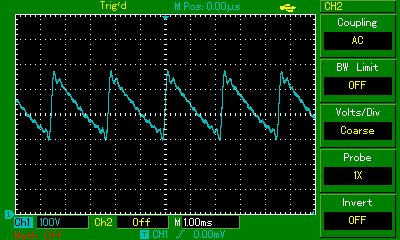
\includegraphics[width=0.7\linewidth]{../../MAP018}
	\caption{Sägezahnspannung: Kanäle zusammengeschaltet}
	\label{fig:map018}
\end{figure}

\subsubsection{Rechteckspannung}
In der Tabelle \ref{tab:RechteckSynthese} befinden sich die theoretisch einzustellenden Werte sowie das theoretische Verhältnis errechnet mit Hilfe der Formel \ref{eqn:theoVerhalt}. Das Ergebnis ist in der Abbildung \ref{fig:map005jpg} zu sehen.
\begin{table}[htbp]
	\centering
	\caption{Theoretischen Daten für Rechteck und theoretisches Verhältnis in Prozent}
	\label{tab:RechteckSynthese}
	\begin{tabular}{c c c}
		\toprule
		$n$ & theoretische $U$/$V$ & theoretisches Verhält. \\
		\midrule
		1 & 0,678 & 100 \\
 		3 & 0,226 & 33,33 \\
		5 & 0,135 & 20,00 \\ 
		7 & 0,096 & 14,29 \\
		9 & 0,075 & 11,11 \\
		\bottomrule
	\end{tabular}
\end{table}
\FloatBarrier
\begin{figure}[htb]
	\centering
	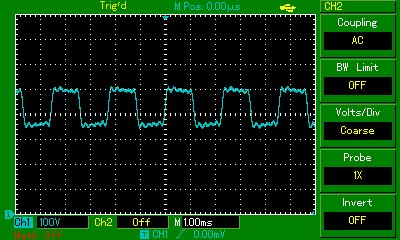
\includegraphics[width=0.7\linewidth]{../../MAP005_jpg}
	\caption{Rechteckspannung: Kanäle zusammengeschaltet}
	\label{fig:map005jpg}
\end{figure}
\subsubsection{Dreiecksspannung}
In der Tabelle \ref{tab:DreieckSynthese} befinden sich ebenfalls theoretisch einzustellenden Werte sowie das theoretische Verhältnis errechnet mit Hilfe der Formel \ref{eqn:theoVerhalt}. Das Ergebnis ist in der Abbildung \ref{fig:map008} zu sehen.
\begin{table}[htbp]
	\centering
	\caption{Theoretischen Daten für Dreieck und theoretisches Verhältnis in Prozent}
	\label{tab:DreieckSynthese}
	\begin{tabular}{c c c}
		\toprule
		$n$ & theoretische $U$/$V$ & theoretisches Verhält. \\
		\midrule
		1 & 0,678 & 100 \\
		3 & 0,075 & 11,11 \\
		5 & 0,027 & 4,00 \\ 
		\bottomrule
	\end{tabular}
\end{table}
\FloatBarrier
\begin{figure}[htb]
	\centering
	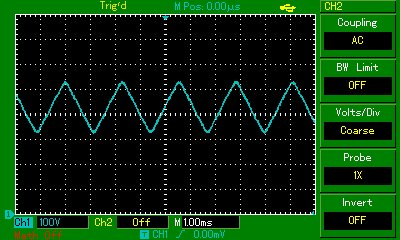
\includegraphics[width=0.7\linewidth]{../../MAP008}
	\caption{Dreieckspannung: Kanäle zusammengeschaltet}
	\label{fig:map008}
\end{figure}
